\subsection{Die Welt der Galaxien}
\begin{itemize}
	\item Erkenntnis, dass die Milchstraße nur eine Galaxie von viele ist $\sim \num{100}$ Jahre alt\\
		vorher: Katalog von Charles Messier (1730-1817)\\
		enthält 103 diffuse Objekte (z.B. M31: Andromeda-Galaxie)\\
		19. Jhd.: NGC=New General Catalogue, John Preyer (1852-1926)\\
		1925: Beobachtung von Cepheiden in M31 durch Edwin Hubble\\
		\begin{itemize}
			\item $D=\SI{285}{k\ps}$ (Aktueller: $\SI{770}{k\ps}$)
		\end{itemize}
		1928: Beobachtung des Auseinanderstrebens der Galaxien
		\begin{itemize}
			\item[] Hubble'sche Gesetz:
				\begin{equation*}
					v=H_0\cdot r \text{ mit } H_0\simeq \SI{72}{\frac{\km}{\s}\cdot\frac{1}{M\ps}} \text{ der Hubble'schen Konstante}
				\end{equation*}
		\end{itemize}
	\item Morphologische Klassifizierung (Hubble-Sequenz)
		\begin{figure}[H]
			\begin{multicols}{2}
				\begin{figure}[H]
					\centering
					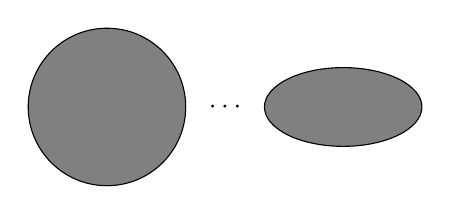
\begin{tikzpicture}
						\draw[fill=black!50!white] (0,0)circle(1cm);
						\node at (1.5,0){$\cdots$};
						\draw[fill=black!50!white,xshift=3cm] (0,0)ellipse(1cm and 0.5cm);
					\end{tikzpicture}
					\caption{$E_0\cdots E_7$}
				\end{figure}\columnbreak
				\begin{figure}[H]
					\centering
					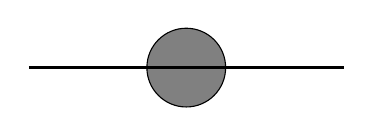
\begin{tikzpicture}
						\draw[fill=black!50!white] (0,0)circle(0.5cm);
						\draw[thick] (-2,0)--(2,0);
					\end{tikzpicture}
					\caption{$S_0$}
				\end{figure}
			\end{multicols}
			\begin{multicols}{3}
				\begin{figure}[H]
					\centering
					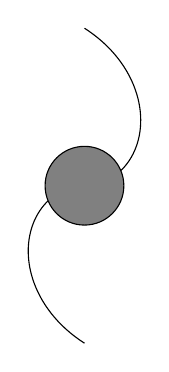
\begin{tikzpicture}
						\draw[domain=0:90,samples=50] plot({\x*cos(\x)/45},{\x*sin(\x)/45})plot({\x*cos(\x+180)/45},{\x*sin(\x+180)/45});
						\draw[fill=black!50!white] (0,0)circle(0.5cm);
					\end{tikzpicture}
					\caption{$S_a$}
				\end{figure}\columnbreak
				\begin{figure}[H]
					\centering
					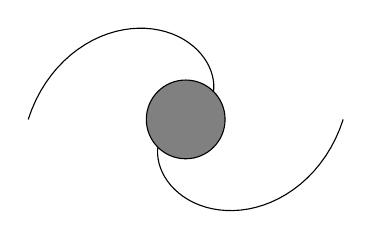
\begin{tikzpicture}
						\draw[domain=0:180,samples=50] plot({\x*cos(\x)/90},{\x*sin(\x)/90})plot({\x*cos(\x+180)/90},{\x*sin(\x+180)/90});
						\draw[fill=black!50!white] (0,0)circle(0.5cm);
					\end{tikzpicture}
					\caption{$S_b$}
				\end{figure}\columnbreak
				\begin{figure}[H]
					\centering
					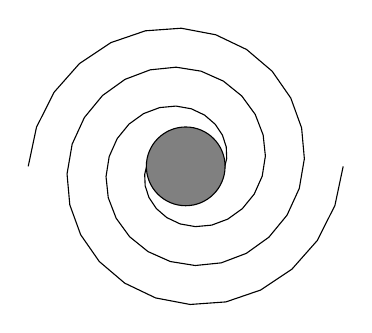
\begin{tikzpicture}
						\draw[domain=0:720,samples=50] plot({\x*cos(\x)/360},{\x*sin(\x)/360})plot({\x*cos(\x+180)/360},{\x*sin(\x+180)/360});
						\draw[fill=black!50!white] (0,0)circle(0.5cm);
					\end{tikzpicture}
					\caption{$S_c$}
				\end{figure}
			\end{multicols}
			\begin{multicols}{3}
				\begin{figure}[H]
					\centering
					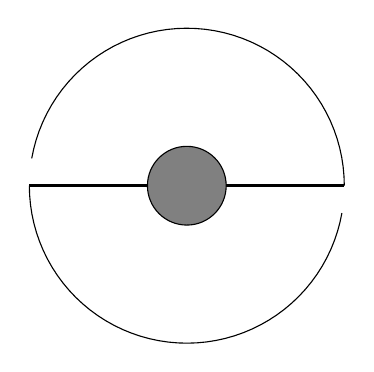
\begin{tikzpicture}
						\draw[very thick] (-2,0)--(2,0);
						\draw[fill=black!50!white] (0,0)circle(0.5cm);
						\draw[domain=0:170,samples=50] plot({2*cos(\x)},{2*sin(\x)})plot({2*cos(\x+180)},{2*sin(\x+180)});
					\end{tikzpicture}
					\caption{$S_{B_a}$}
				\end{figure}\columnbreak
				\begin{figure}[H]
					\centering
					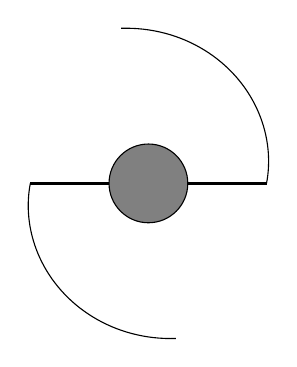
\begin{tikzpicture}
						\draw[very thick] (-1.5,0)--(1.5,0);
						\draw[fill=black!50!white] (0,0)circle(0.5cm);
						\draw[domain=0:100,samples=50] plot({(\x/200+1.5)*cos(\x)},{(\x/200+1.5)*sin(\x)})plot({(\x/200+1.5)*cos(\x+180)},{(\x/200+1.5)*sin(\x+180)});
					\end{tikzpicture}
					\caption{$S_{B_b}$}
				\end{figure}\columnbreak
				\begin{figure}[H]
					\centering
					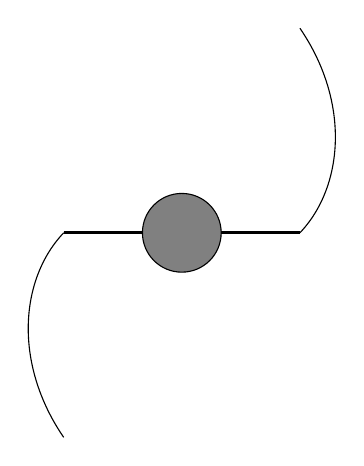
\begin{tikzpicture}
						\draw[very thick] (-1.5,0)--(1.5,0);
						\draw[fill=black!50!white] (0,0)circle(0.5cm);
						\draw[domain=0:60,samples=50] plot({(\x/40+1.5)*cos(\x)},{(\x/40+1.5)*sin(\x)})plot({(\x/40+1.5)*cos(\x+180)},{(\x/40+1.5)*sin(\x+180)});
					\end{tikzpicture}
					\caption{$S_{B_c}$}
				\end{figure}
			\end{multicols}
		\end{figure}
		\begin{itemize}[label={}]
			\item Elliptische Galaxien E
			\item Spiralgalaxien mit und ohne Balken (S,S\textsubscript{B})
			\item Irreguläre Galaxien I
			\item Milchstraße S\textsubscript{B\textsubscript{bc}}
		\end{itemize}
\end{itemize}
\subsubsection{Elliptische Galaxien Allgemein}
Normale Ellipsen: $E$ mit Elliptizität $0\leq\epsilon\leq\num{0.7}$\\
$E_n$ wobei $n=\SI{10}{\epsilon}\Rightarrow E_0-E_7$
\begin{itemize}
	\item $S_0$ Galaxien: Übergang zwischen Elliptischen und Spiralgalaxien (linsenförmig mit Bulge und Scheibe ohne Spiralarme)
	\item CD Galaxien elliptische Riesengalaxien
		\begin{table}[H]
			\begin{tabular}{p{3cm}|p{3cm}|p{3cm}|p{3cm}}
				& $E$ & $S_0$ & $CD$ \\\hline
				Absolute Helligkeit & $-\num{15}-(-\num{23})$ & $(-\num{17})-(-\num{22})$ & $(-\num{22})-(-\num{25})$ \\\hline
				$\frac{M}{M_0}$ & $\num{100}-10^{13}$ & $10^{10}-10^{12}$ & $10^{13}-10^{14}$ \\\hline
				$\frac{2R}{\si{k\ps}}$ & $\num{1}-\num{200}$ & $\num{10}-\num{100}$ & $\num{300}-\num{1000}$ \\\hline
				$\frac{\frac{M}{L_B}}{\frac{M_\odot}{L_\odot}}$ & $\num{10}-\num{100}$ & $\sim\num{10}$ & $>\num{100}$
			\end{tabular}
		\end{table}
	\item Leuchtkraft: de Vancouleurs-Profil: $\log\left(\frac{I(R)}{I_0}\right)=-\num{3.3307}\left(\left(\frac{R}{R_e}\right)^\frac{1}{4}-1\right)$\\
		$I(R)$: Flächenhelligkeit in $\frac{L_\odot}{\si{\ps^2}}$\\
		$R_l$: Effektivradius, mit $\int\limits_0^{R_l}dRR_I(R)=\frac{1}{2}\int\limits_0^\infty dR R_I(R)$
	\item woher kommt die Abplattung der Elliptischen Galaxie?
		\begin{enumerate}[label={$\roman*)$}]
			\item Rotation? In diesem Fall gelte: $\frac{rot}{\sigma}\approx\sqrt{\frac{\epsilon}{1-\epsilon}}$\\
				\textbf{Aber}: Beobachtet $v_r\ <<\sigma$
			\item Selbst gravitierendes Gleichgewichtssystem (Elliptizität ergibt sich aus den Anfangsbedingungen) Zeitlich stabil? $\to$ "`thermalisierung"' durch 2er Stöße?
		\end{enumerate}
	\item Betrachte Relaxationszeit druch 2er Stöße in einem System von $N$ Sternen der Masse $m$ (Gesamtmasse $M=N\cdot m$) der Ausdehnung $R$: $t_{relax}=\frac{R}{v}\cdot\frac{N}{\ln(N)}=\underset{\underset{\underset{\text{eines Sterns beim durchqueren}}{\text{charakteristische Zeit}}}{\uparrow}}{t_{cross}}\cdot\frac{N}{\ln(N)}$\\
		charakteristische Zeit, in der ein Stern durch 2er-Stöße  seine Richtung um $\SI{90}{\degree}$ ändert\\
		für eine Galaxie $N\sim 10^{12}, t_{cross}\approx 10^8\si{a}\Rightarrow t_{relax}\approx\SI{14e9}{a}$ (älter als Universum) $\Rightarrow $ stabil
\end{itemize}
\subsubsection{Spiralgalaxien}
\begin{table}[H]
	\def\k{2.3cm}
	\begin{tabular}{p{\k}|p{\k}|p{\k}|p{\k}|p{\k}}
		& $S_a$ & $S_b$ & $S_c$ & $S_{d}$ \\\hline
		$M_B$ & $-\num{17}-(-\num{23})$ & $-\num{17}-(-\num{23})$ & $(-\num{10})-(-\num{22})$ & $(-\num{15}-(-\num{20})$ \\\hline
		$\frac{M}{M_\odot}$ & $10^9-10^{12}$ & $10^9-10^{12}$ & $10^9-10^{12}$ & $10^8-10^{10}$ \\\hline
		$\frac{\frac{M}{L_B}}{\frac{M_\odot}{L_\odot}}$ & $\num{6.0}\pm\num{0.6}$ & $\num{4.5}\pm\num{0.4}$ & $\num{2.6}\pm\num{0.2}$ & $-\num{1}$ \\\hline
		$\frac{L_{Bulge}}{L_{tot}}$ & $\num{0.3}$ & $\num{0.13}$ & $\num{0.05}$ & - \\\hline
		$\frac{2R}{\si{k\ps}}$ & $\num{5}-\num{100}$ & $\num{5}-\num{100}$ & $\num{5}-\num{100}$ & $\num{0.5}-\num{50}$ \\\hline
		$\frac{v_{max}}{\left(\si{\frac{\km}{\s}}\right)}$ & $\num{300}$ & $\num{220}$ & $\num{175}$ & - 
	\end{tabular}
\end{table}
Profil des Bulges folgt einem de Vancouleurs-Profil:\\
Mit Flächenhelligkeit $U\sim\num{2.5}\log(I):$\\
$M_{Bulge}(R)=U_e+\num{8.326}\cdot\left(\left(\frac{R}{R_e}\right)^\frac{1}{4}-1\right)$\\
$M_{Scheibe}(R)=U_0+\num{1.09}\left(\frac{R}{n_R}\right)$\\
Ian Freeman: $U_0$ ist konstant für verschiedene Spiralgalaxien\\
$S_a-S_c$: $U_0=\num{21.5}\pm\SI{0.39}{\frac{\text{mag}}{\text{arc}\s^2}}$\\
$S_d$: $U_0=\num{22.07}\pm\SI{0.4}{\frac{\text{mag}}{\text{arc}\s^2}}$
\begin{itemize}
	\item Rotationsachsen von Spiralgalaxien verlaufen nicht wie durch die Lichtverteilung erwartet für $R\geq n_R$, sondern im wesentlichen flach, (vgl. Kap 3.3)
		\begin{itemize}
			\item Spiralgalxien sind von einem Halo dunkler Materie umgeben!\\
				Es gilt (Gleichgewicht zwischen Zentrifugal- und Gravitationskraft):
				\begin{equation*}
					V^2(R)=\frac{G\cdot M(R)}{R} \quad\text{Gesamtmasse von $R$}
				\end{equation*}
				für sichtbare Materie:
				\begin{equation*}
					V^2_{enm}=\frac{GM_{enm}(R)}{R} \ \Rightarrow\ V^2_{dark}=V^2-V_{enm}^2=\frac{G\cdot M_{dark}}{R}
				\end{equation*}
			\item $M_{dark}(R)=\frac{R}{G}\left(V^2(R)-V^2_{enm}(R)\right)$
				\begin{itemize}[label={\textbullet}]
					\item Problem: äußerer Radius ist Halo und daher nicht klar\\
						Sterne: $R\geq\SI{40}{k\ps}$\\
						Satelliten: $R\geq\SI{140}{k\ps}$
				\end{itemize}
				Zusammensetzung:
				\begin{itemize}[label={}]
					\item Elliptische Galaxien: alte Sterne (orange und rot)
					\item Spiralgalaxien: Bulge ähnlich wie elliptische Galaxien, Spiralarme mit geringem blauanteil
				\end{itemize}
		\end{itemize}
\end{itemize}
\subsubsection{Skalengesetze}
Tully-Fisher (177)
\begin{equation*}
	L\sim V^4_{max}
\end{equation*}
\begin{itemize}[label={$\cdot$}]
	\item Korrelation zwischen maximaler Rotationsgeschwindigkeit von Spiralen und Leuchtkraft
		\begin{itemize}
			\item recht genaue Abschätzung der Leuchtkraft aus der Rotationskurve der Galaxie
		\end{itemize}
	\item Durch Vergleich mit scheinbarer Helligkeit $\Rightarrow$ Abstand
	\item heuristische Herleitung:\\
		Rotationskurve bei $V(R)=const. $ impliziert
		\begin{equation*}
			M=\frac{V_{max}^2\cdot R}{G}\ \Rightarrow\ L=\left(\frac{M}{L}\right)^{-1}\cdot\frac{V_{max}\cdot R}{G}
		\end{equation*}
		mittlere Flächenhelligkeit: $\langle I\rangle = \frac{L}{R^2}$
		\begin{equation*}
			\Rightarrow L=\left(\frac{M}{L}\right)^{-1}\cdot\frac{V_{max}\cdot R}{G\cdot M}\cdot\frac{V_{max}\cdot R}{G}=\left(\frac{M}{L}\right)^{-2}\cdot\frac{V_{max}}{G}\cdot\frac{1}{\langle I\rangle}
		\end{equation*}
		Freeman: $\langle I\rangle\sim cnst.$ für Spiralgalaxien\\
		$\frac{M}{L}$ variiert nur wenig $\Rightarrow\ L\sim V_{max}^4$\\
		(kein Beweis, aber macht Skalengesetz plausibel)
\end{itemize}
